\chapter{Resultados}
\label{chap:resultados}
A fase de desenvolvimento do robô Doogie culminou em 4 resultados principais: Protótipo, ambiente de simulação e a estrutura de software da plataforma móvel. Os tópicos posteriores irão detalhar cada um desses resultados. 

%--------- NEW SECTION ----------------------
\section{Protótipo}
\label{sec:resultado_prototipo}
O protótipo é composto por duas placas (placa inferior e placa superior) resultantes da integração de componentes eletrônicos. Na Figura \ref{fig:top_board_elementos}, é possível visualizar alguns dos componentes eletrônicos que compõem a placa superior, quais sejam: a IMU que é responsável por fornecer dados que auxiliam no processo de localização do Doogie dentro do labirinto, os LEDs, Buzzer, Push Buttons que têm por finalidade garantir a interface do usuário com o robô, promovendo indicações luminosas e sonoras. O \textit{Pin Header} da Raspberry que é a conexão física da placa com a própria Raspberry, o Multiplexador Analógico e o Conversor A/D que interagem entre si permitindo a aquisição dos dados dos sensores e da bateria em formato analógico, transformando-os em digital e, por fim, o conversor DC-DC 5V que garante que a tensão de alimentação da Raspberry mantenha-se conforme especificação (5V). Vale ressaltar que o \textit{Pin Header} macho é responsável por permitir a conexão entre as placas inferior e superior.

\begin{figure}[H]
	\centering
	\caption{Componentes da placa superior do Doogie Mouse}
	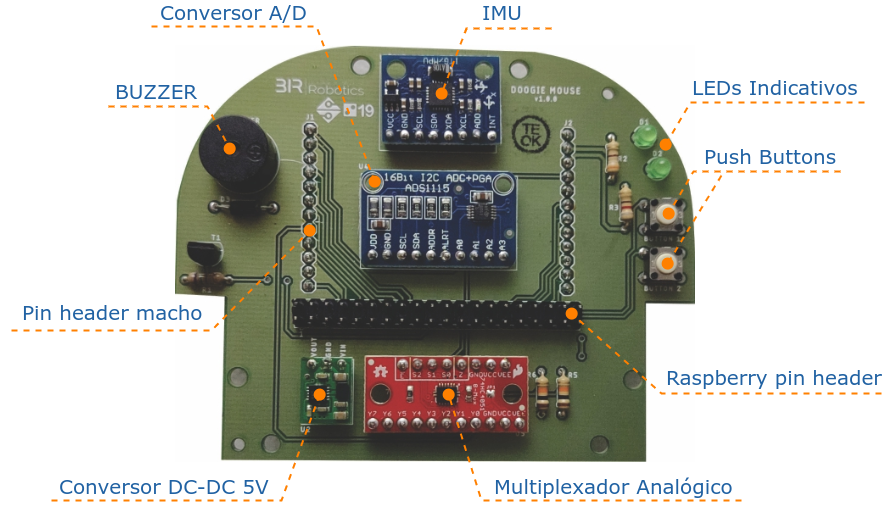
\includegraphics[width=1\textwidth]
	{Figures/top_board_elementos.png}
	\label{fig:top_board_elementos}
	\source{Própria Autoria}
\end{figure}

Sabendo sobre a funcionalidades dos componentes da placa superior, podemos observar agora a figura \ref{fig:bottom_board_elementos}. Os componentes que compõem a placa inferior, cuja parte circulada em cor vermelha refere-se ao conjunto do motor que é formado pelas rodas, \textit{bracket}, micro motor, encoder magnético, \textit{flat cable} e conector IDC fêmea. Esse conjunto é responsável por garantir o correto acionamento e funcionamento do motor, promovendo suas interligações elétricas e mecânicas, fornecendo dados para aprimorar o sistema de controle do motor. É possível identificar 4 pares de sensores infra-vermelho (Emissor IR e Fototransistor) na placa inferior, que são responsáveis por identificar os obstáculos próximos ao robô. Observa-se também o conversor DC-DC 6V que tem função de fornecer para os sensores e motores a tensão necessária para o funcionamento dos mesmos, o componente Ponte H que permite o controle de sentido de giro do eixo dos motores bem com a potência elétrica, as chaves Liga/Desliga que ligam e desligam os circuitos da bateria e dos motores, o conector da bateria que é responsável pela fixação da bateria e o próprio componente bateria que é responsável por fornecer a tensão de alimentação para o funcionamento de ambas as placas. A integração das placas inferior e superior juntamente com a Raspberry é o que compõem o protótipo físico do robô Doogie Mouse (vide Figura \ref{fig:prototipos}).

\begin{figure}[H]
	\centering
	\caption{Componentes da placa inferior do Doogie Mouse}
	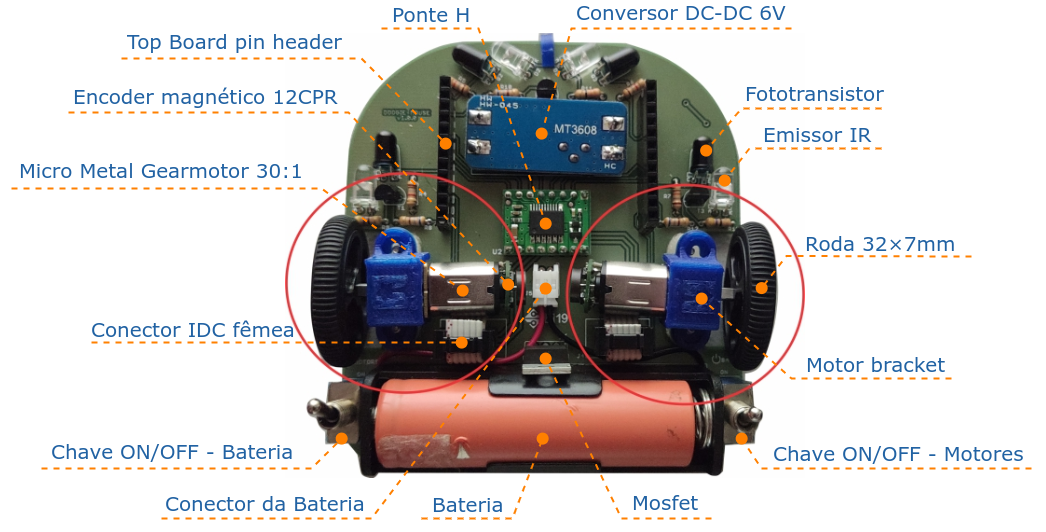
\includegraphics[width=1\textwidth]
	{Figures/bottom_board_elementos.png}
	\label{fig:bottom_board_elementos}
	\source{Própria Autoria}
\end{figure}

\begin{figure}[H]
	\centering
	\caption{Protótipos do Doogie Mouse confeccionados}
	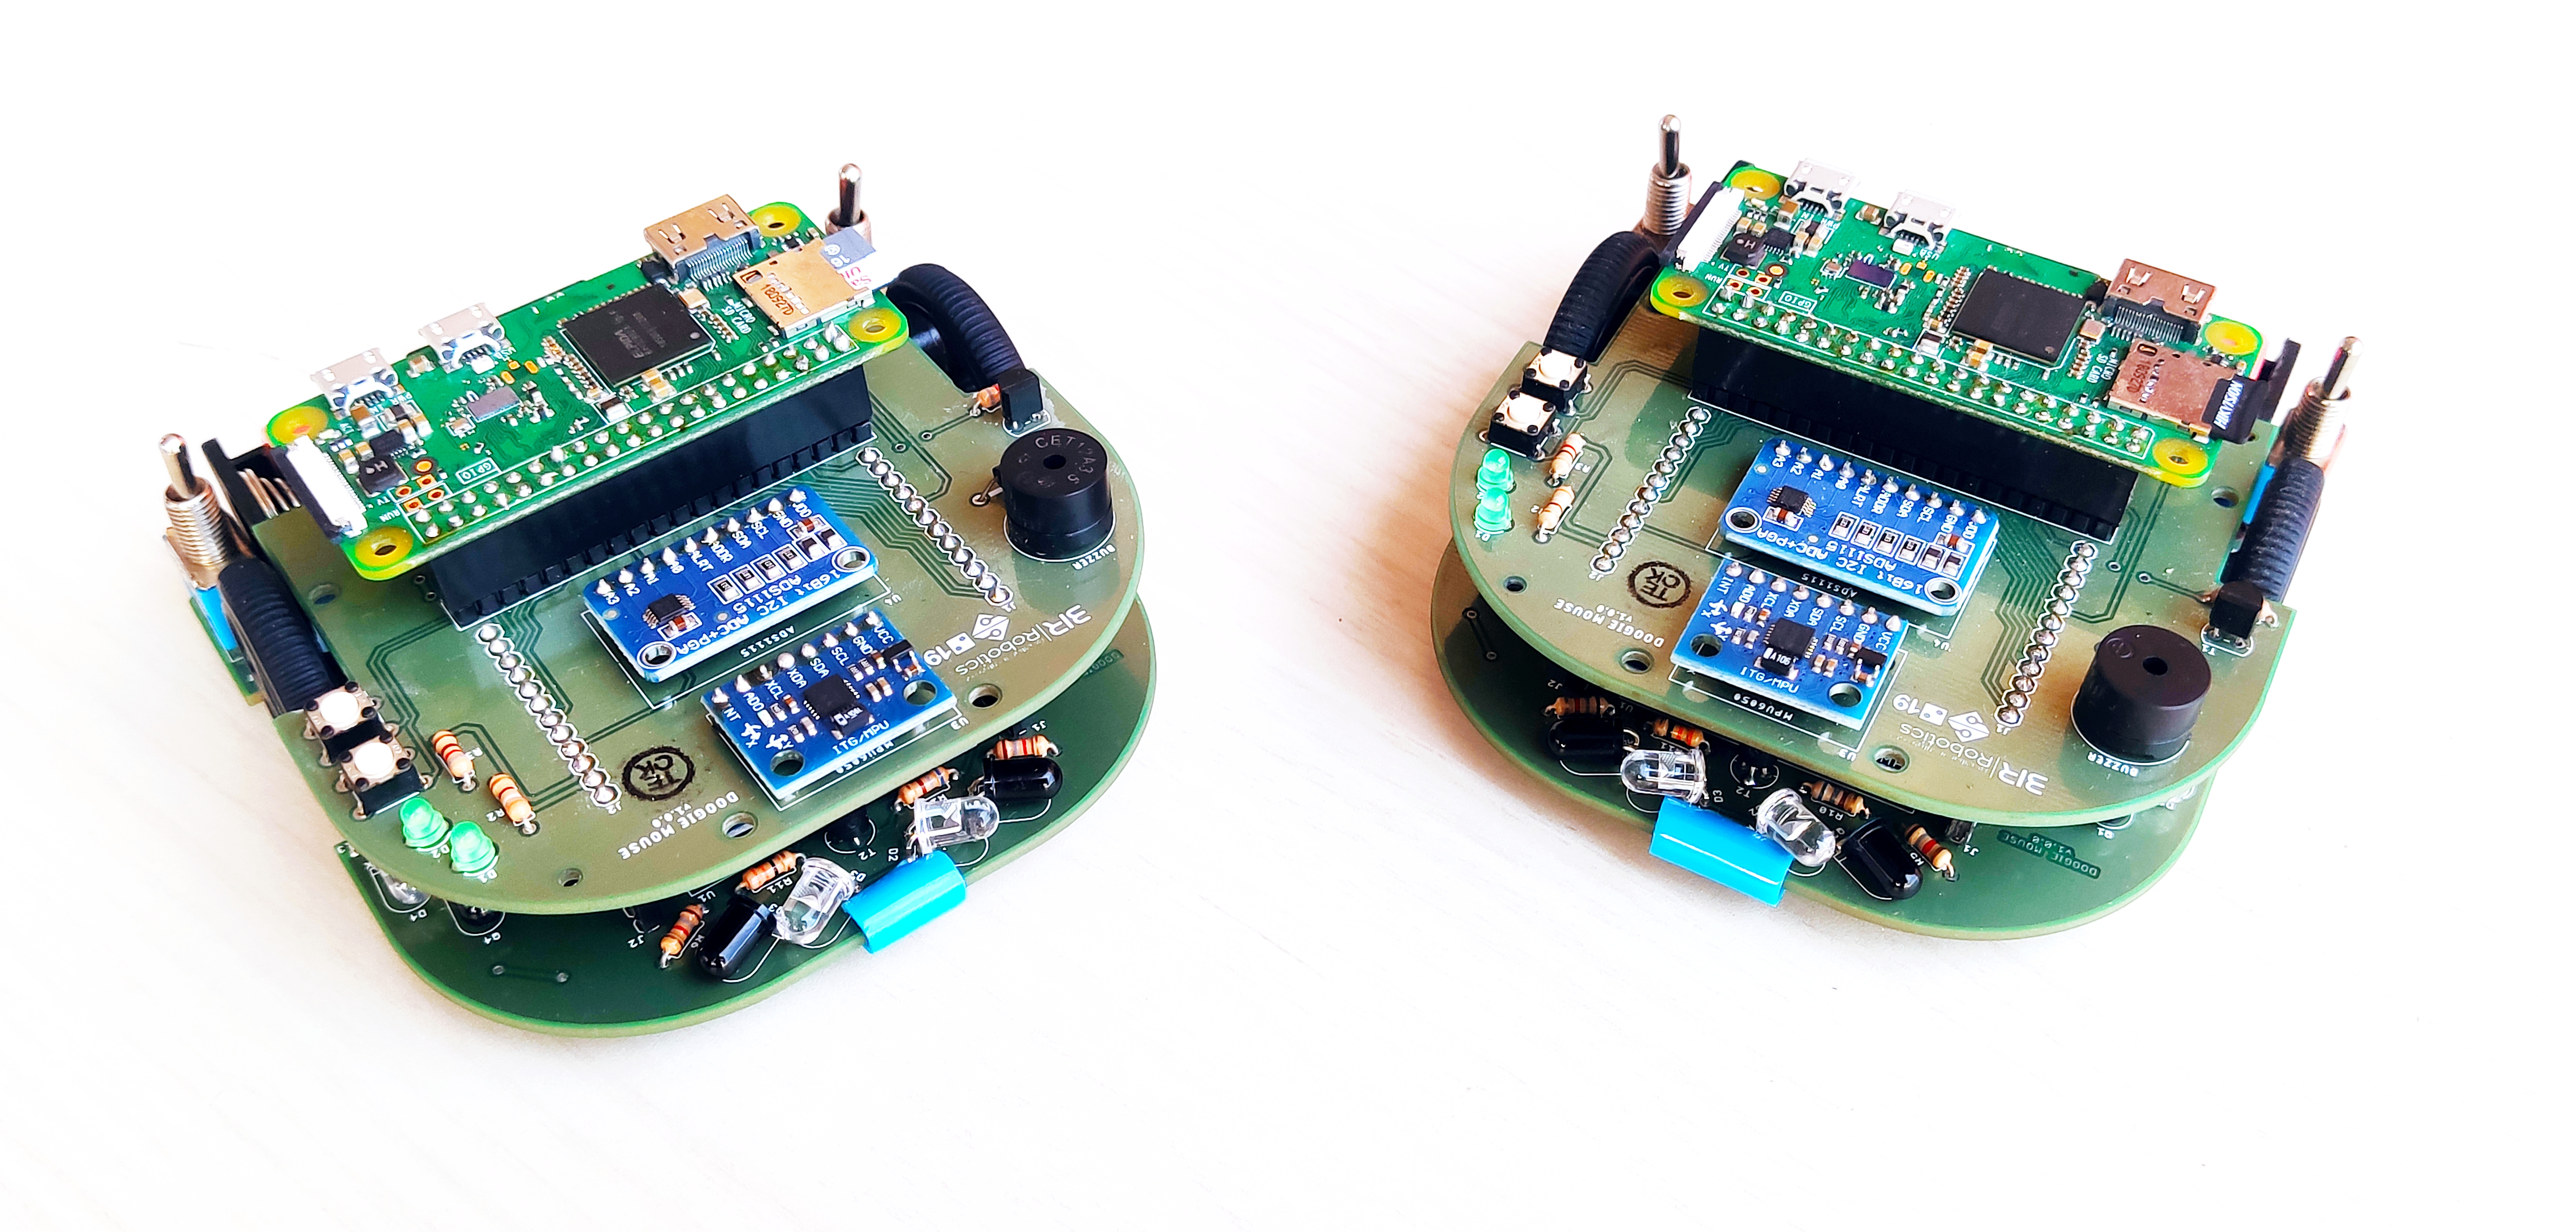
\includegraphics[width=1\textwidth]
	{Figures/doogie_mouse_prototipos}
	\label{fig:prototipos}
	\source{Própria Autoria}
\end{figure}

Visando auxiliar os usuários, o protótipo dispõe de dois guias: um guia de montagem das placas e um guia de configuração de software. O guia de montagem das placas está disponível no site GitHub para acesso por qualquer usuário. Esse guia foi criado para proporcionar ao usuário uma experiência didática com relação à parte de hardware do Doogie e apresenta uma sequência de passos para fixação dos componentes eletrônicos, assim como algumas dicas, que tem por objetivo garantir mais facilidade no decorrer do processo de montagem. Nesse documento também são listados os requisitos físicos necessários para montagem do robô, bem como, ferramentas utilizadas, componentes eletrônicos e os equipamentos de proteção individual (EPI’s), aconselháveis utilização durante todo o procedimento para evitar qualquer tipo de acidente. Com o intuito de eliminar possíveis dúvidas durante as etapas de montagem, o documento supracitado dispõe de imagens que ilustram detalhadamente todo passo a passo de fixação de cada componente. Uma parte desse guia, que possui mais de 34 passos de montagem,  pode ser visualizado na Figura \ref{fig:guia_hardware_setup}.

\begin{figure}[H]
	\centering
	\caption{Recorte do guia de instruções de montagem do Doogie Mouse}
	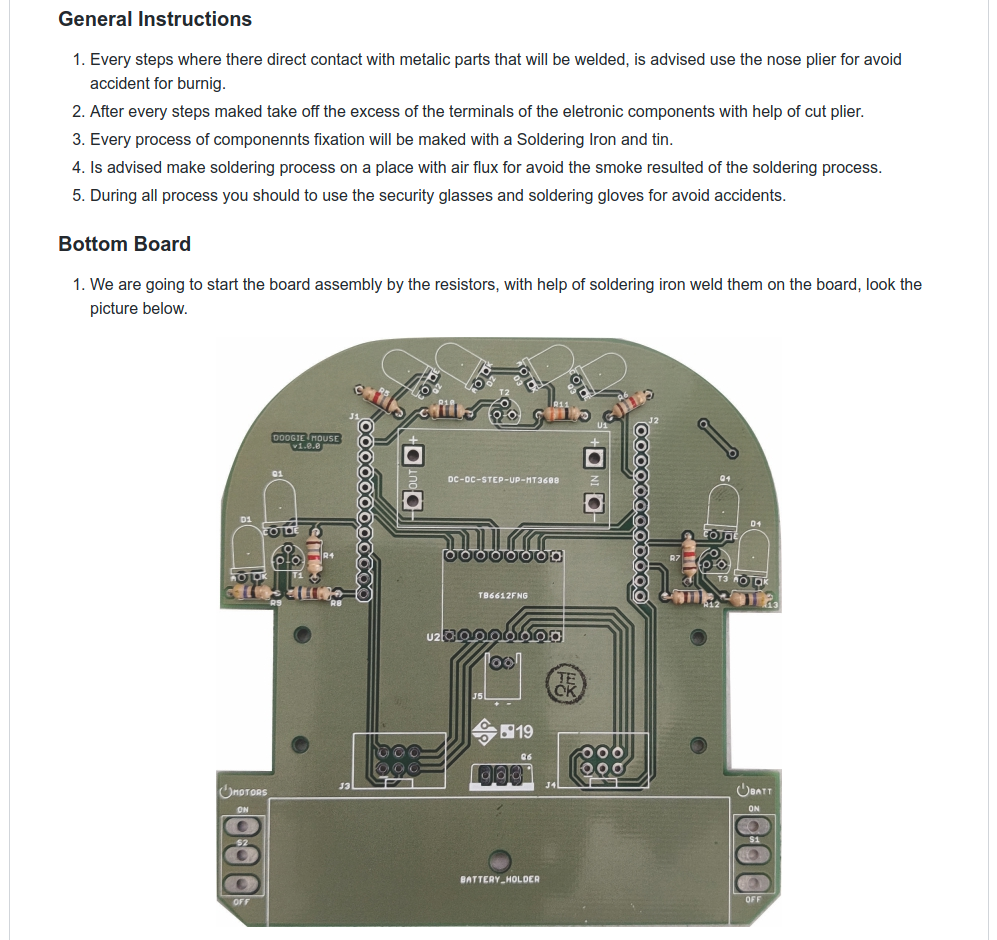
\includegraphics[width=0.9\textwidth]
	{Figures/guia_hardware_setup}
	\label{fig:guia_hardware_setup}
	\source{Própria Autoria}
\end{figure}

De maneira análoga ao guia de montagem das placas, o guia de configuração de software também está disponível no GitHub, conforme ilustrado pela Figura \ref{fig:guia_software_setup}. O manual de configuração de software informa sobre os requisitos físicos necessário para iniciar as configurações e apresenta uma lista com as instruções sobre instalação e resolução de dependência de todos os softwares necessários para o funcionamento do Doogie, que varia desde a preparação da unidade de armazenamento em que é instalado o sistema operacional até um código teste dentro do ambiente do ROS. Esse manual também dispõe de uma galeria de imagens ilustrando as telas de acordo com cada procedimento, garantindo ao usuário um ótimo entendimento das etapas.

\begin{figure}[H]
	\centering
	\caption{Recorte do guia de instruções de configuração de software do Doogie Mouse}
	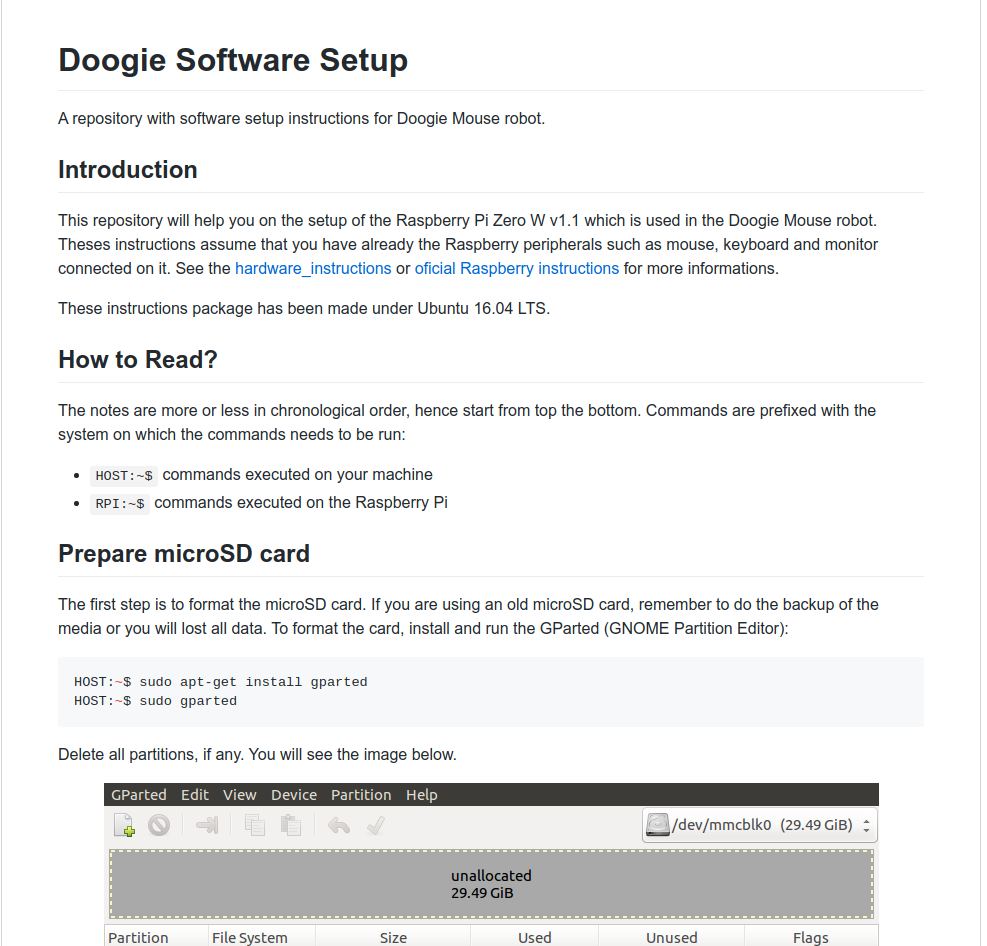
\includegraphics[width=1\textwidth]
	{Figures/guia_software_setup}
	\label{fig:guia_software_setup}
	\source{Própria Autoria}
\end{figure}

\section{Ambiente de simulação}
\label{sec:resultado_ambiente_de_simulacao}
\subsection{Comparativo de Malhas}
\label{ssec:comparativo_de_malhas}
No comparativo de malhas, analisou-se como os formatos \gls{collada} (.dae) e \gls{stl}(.stl) interferem na simulação, bem como o uso de tipos primitivos para a representação da malha de colisão. Na Tabela \ref{tab:ComparativoMalhas}, comparam-se os modelos simplificados, gerado na seção \ref{sec:Simulacao}, usando malhas em \gls*{collada} (Doogie\_lite\_dae) e \gls*{stl} (Doogie\_lite\_stl), e o modelo 3D sem simplificações (Doogie\_real\_dae) gerado na seção \ref{sec:modelo_mecanico} usando sua malha em \gls*{collada}.

\begin{table}[H]
	\centering
	\caption{Comparativo entre malhas carregadas no Gazebo}
	\begin{tabular}{|l|l|l|l|l|}
		\hline
		& \multicolumn{1}{c|}{\textbf{\begin{tabular}[c]{@{}c@{}}Visual\\ (Faces)\end{tabular}}} & \multicolumn{1}{c|}{\textbf{\begin{tabular}[c]{@{}c@{}}Colisão\\ (Faces)\end{tabular}}} & \multicolumn{1}{c|}{\textbf{FPS}} & \multicolumn{1}{c|}{\textbf{\begin{tabular}[c]{@{}c@{}}Real Time \\ Factor\end{tabular}}} \\ \hline
		\textbf{Doogie\_lite\_dae} & 70.410                                                                                 & 70.410                                                                                  & $\sim$1,5                         & 0,35                                                                                      \\ \hline
		\textbf{Doogie\_real\_dae} & 1.091.337                                                                              & 1.091.337                                                                               & $\sim$0,6                         & 0,03                                                                                      \\ \hline
		\textbf{Doogie\_lite\_stl} & 70.398                                                                                 & 70.398                                                                                  & $\sim$4.2                         & 0,33                                                                                      \\ \hline
	\end{tabular}
	\label{tab:ComparativoMalhas}
	\source{Própria Autoria}
\end{table}

O formato \*gls{collada} possui perfomance na simulação ligeiramente inferior ao \gls*{stl}, principalmente em relação ao \gls*{fps} no qual foi 36\% inferior ao desempenho da outra malha. Também fica visível a necessidade da simplificação do modelo do robô, sendo inviável a simulação do Doogie\_real\_dae que teve seu \gls*{fps} inferior a um e o \gls*{rtf} próximo a zero, denotando uma simulação lenta e de pouca acurácia. 


\begin{table}[H]
	\centering
	\caption{Comparativo com simplificação da malha de colisão}
	\begin{tabular}{|l|l|l|l|l|}
		\hline
		& \multicolumn{1}{c|}{\textbf{\begin{tabular}[c]{@{}c@{}}Visual\\ (Faces)\end{tabular}}} & \multicolumn{1}{c|}{\textbf{\begin{tabular}[c]{@{}c@{}}Colisão\\ (Faces)\end{tabular}}} & \multicolumn{1}{c|}{\textbf{FPS}} & \multicolumn{1}{c|}{\textbf{\begin{tabular}[c]{@{}c@{}}Real Time \\ Factor\end{tabular}}} \\ \hline
		\textbf{Doogie\_lite\_dae} & 70.410                                                                                 & 6                                                                                       & $\sim$8,0                         & 0,52                                                                                      \\ \hline
		\textbf{Doogie\_real\_dae} & 1.091.337                                                                              & 6                                                                                       & $\sim$3,5                         & 0,52                                                                                      \\ \hline
	\end{tabular}
	\label{tab:ComparativoMalhaSimplificada}
	\source{Própria Autoria}
\end{table}

Ao comparar o desempenho como uso do modelo simplificado e o modelo real, usando tipos primitivos para a representação da malha de colisão pode-se perceber que o gargalo da simulação se encontra no número das faces de colisão usadas para a representação dinâmica do robô. A taxa de \gls*{fps} aumentou em seis vezes em relação a análise anterior, atingindo um \gls*{rtf} igual ao do modelo simplificado, conforme visto na Tabela \ref{tab:ComparativoMalhaSimplificada}. Sendo assim a configuração Doogie\_lite\_dae com a simplificação da malha de colisão a mais otimizada para uso na simulação sem perda de cor e textura do modelo do robô.


\subsection{Modelos da Simulação}
\label{sec:modelos_sim}
\begin{figure}[H]
	\centering
	\caption{Doogie Mouse no Gazebo}
	\subfigure[Juntas do robô]{\label{fig:doogie_gazebo_joints}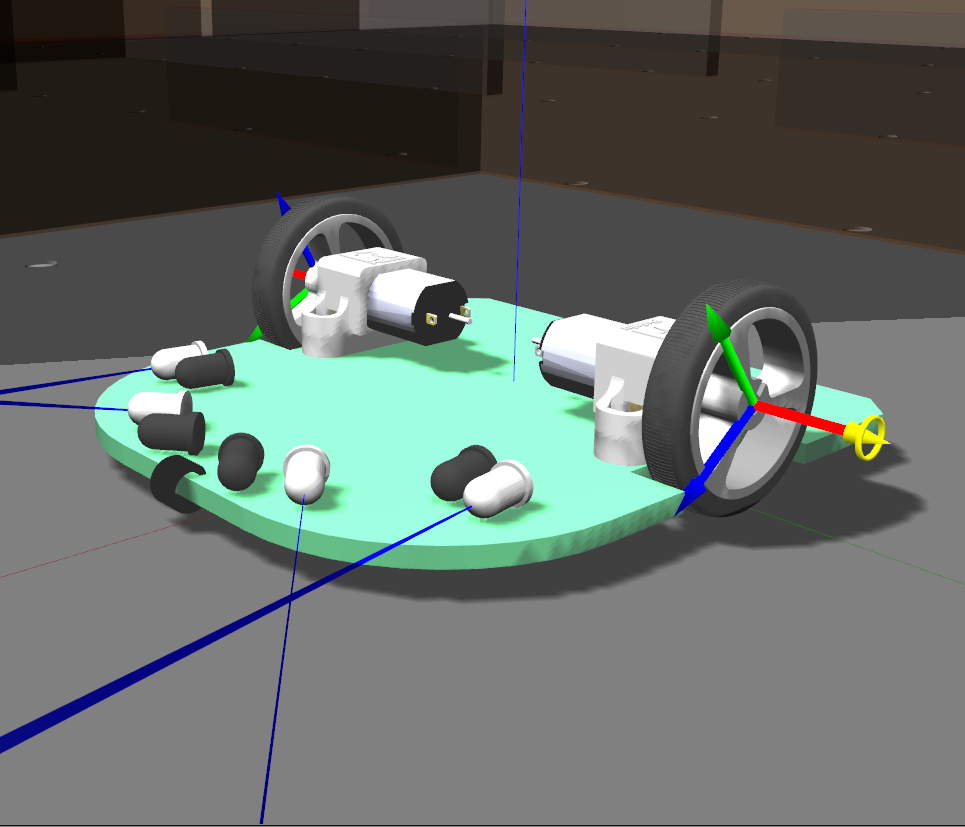
\includegraphics[scale=0.198]{doogie_gazebo_joints}}
	\subfigure[Visualização das transformadas e centro de gravidade]{\label{fig:doogie_gazebo_tfs}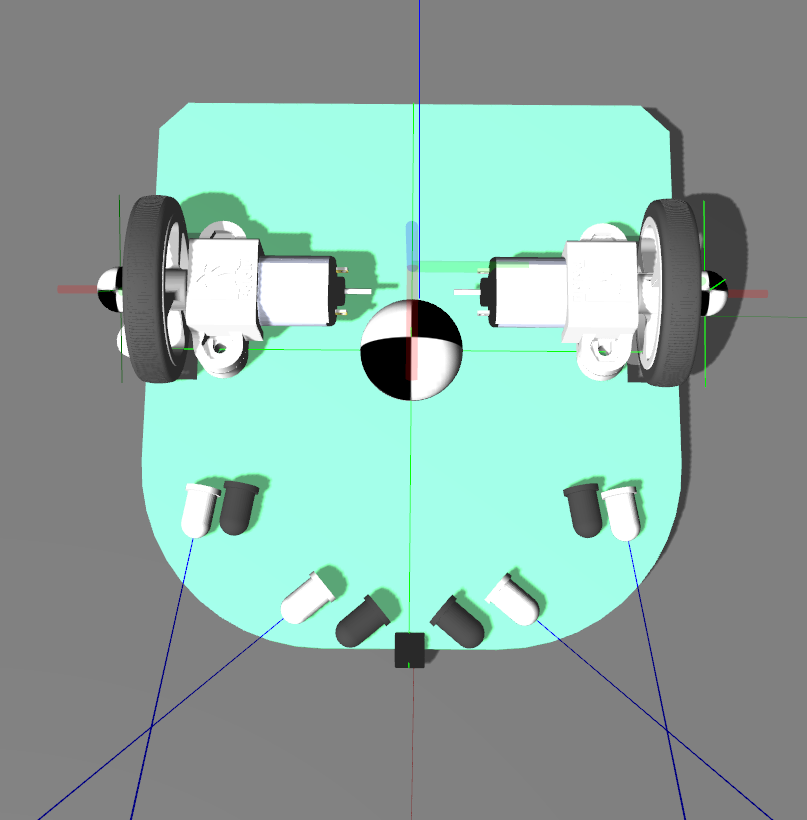
\includegraphics[scale=0.2]{doogie_gazebo_tfs}}
	\subfigure[Modelo renderizado no Gazebo]{\label{fig:doogie_gazebo}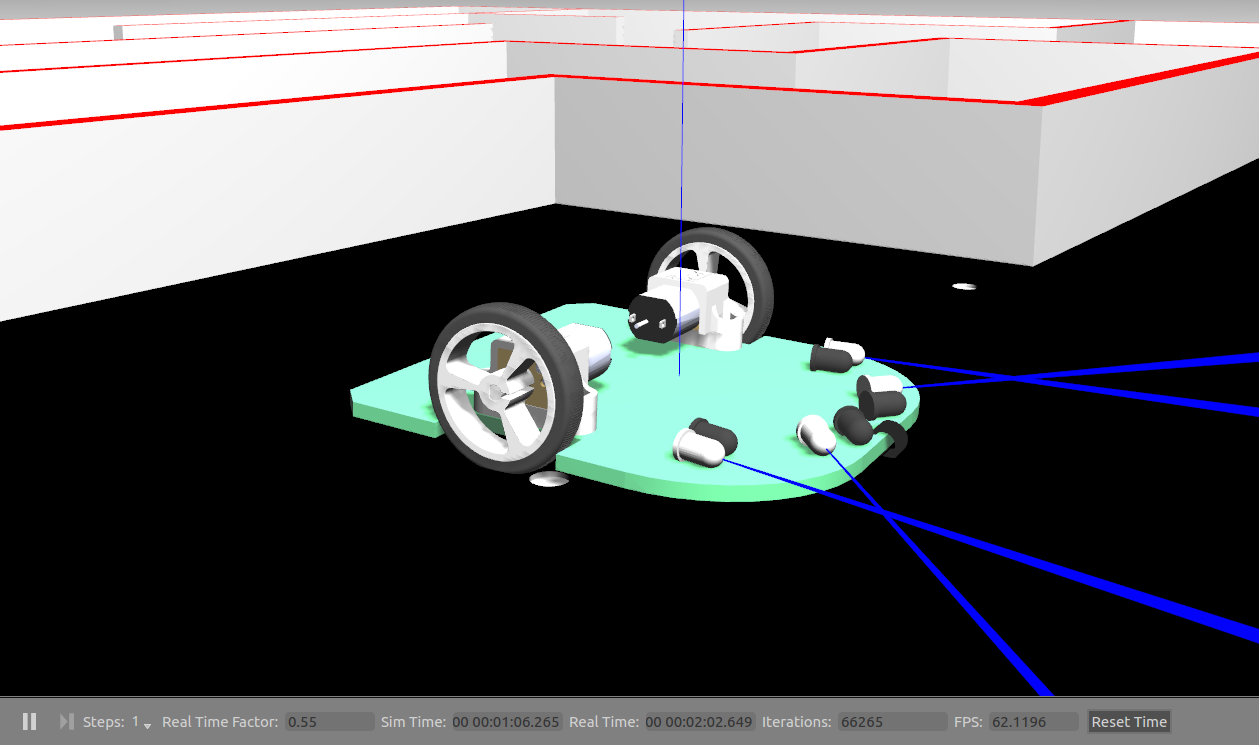
\includegraphics[scale=0.38]{doogie_gazebo}}
	\label{fig:doogie_gazebo_imgs}
\end{figure}
Os modelos exportados para o Gazebo, seguindo a metodologia descrita na seção \ref{sec:Simulacao}, simplificando o modelo 3D gerado pelo SolidWorks, e usando a configuração otimizada obtida no comparativo de malhas da subseção \ref{ssec:comparativo_de_malhas}, do robô e do labirinto foram elaborados de forma a não comprometer a simulação em sua acurácia de ser realizada próxima do tempo real, \gls*{rtf}, ou na sua taxa de atualização de quadros \gls*{fps}. Assim, atingiu-se a simulação simultânea de ambos os modelos, sem comprometimento desses indicadores e em máquinas mais recentes a simulação pode chegar a se manter dentro de 60 \gls*{fps}, a taxa mais comum de de atualização usada nos monitores comerciais.

Dessa forma, provê-se um ambiente de simulação que facilite o acesso dos usuários ao Doogie Mouse, mesmo que para esses não seja possível adquirir a plataforma física, tornando-o mais acessível em sua proposta de ensino.



\label{sec:modelos_sim}
\begin{figure}[H]
	\centering
	\caption{Labirinto na Simulação}
	\subfigure[Labirinto renderizado no Gazebo]{\label{fig:maze_gazebo}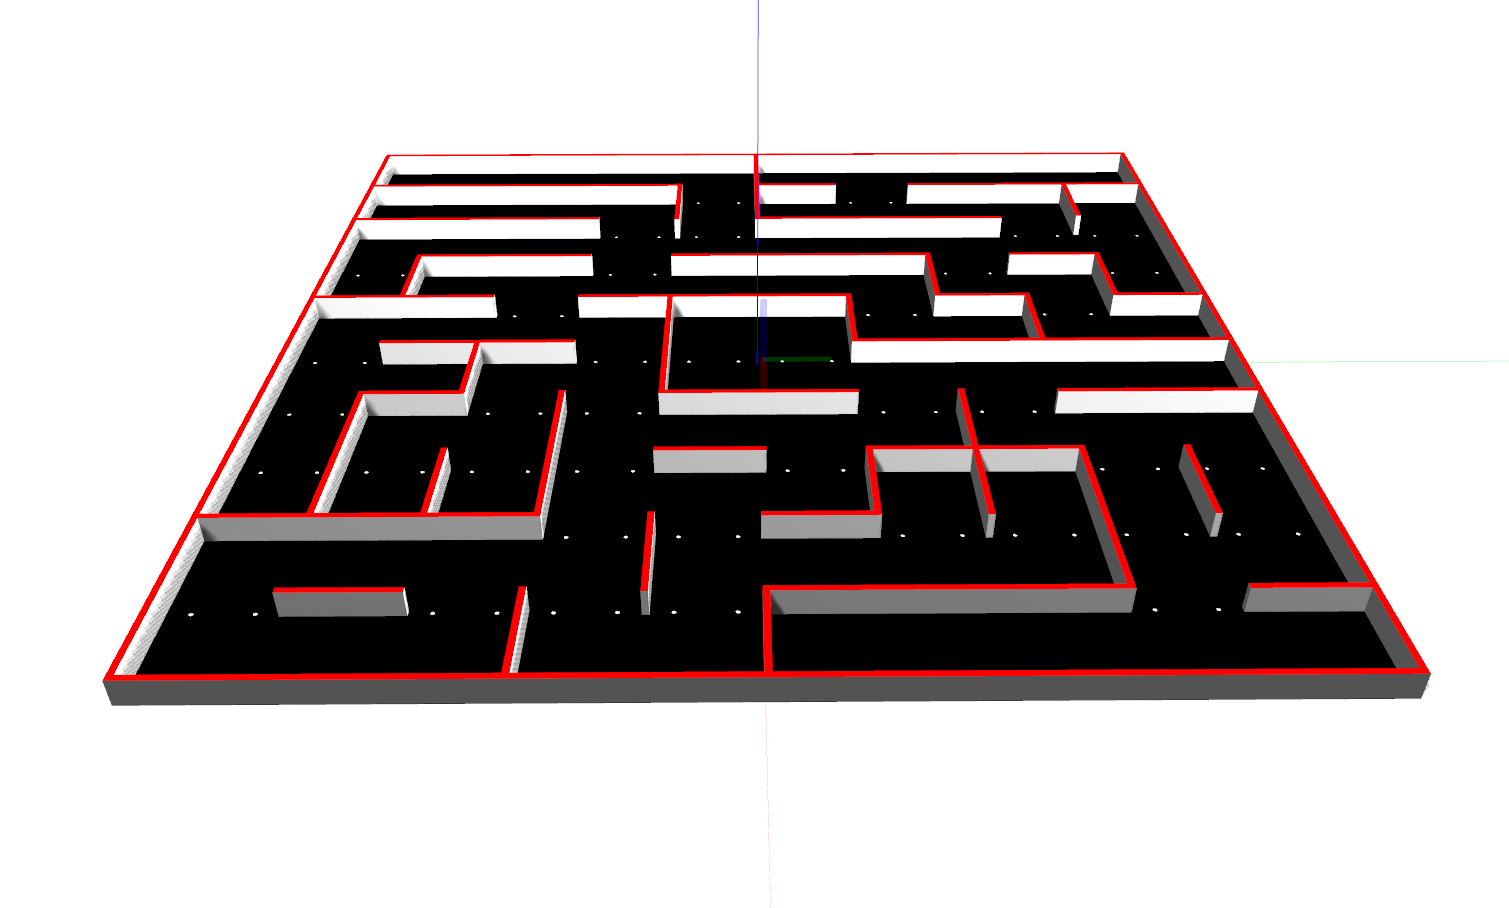
\includegraphics[scale=0.198]{maze_gazebo}}
	\subfigure[Malha de colisão das paredes]{\label{fig:minus_gazebo_colisions}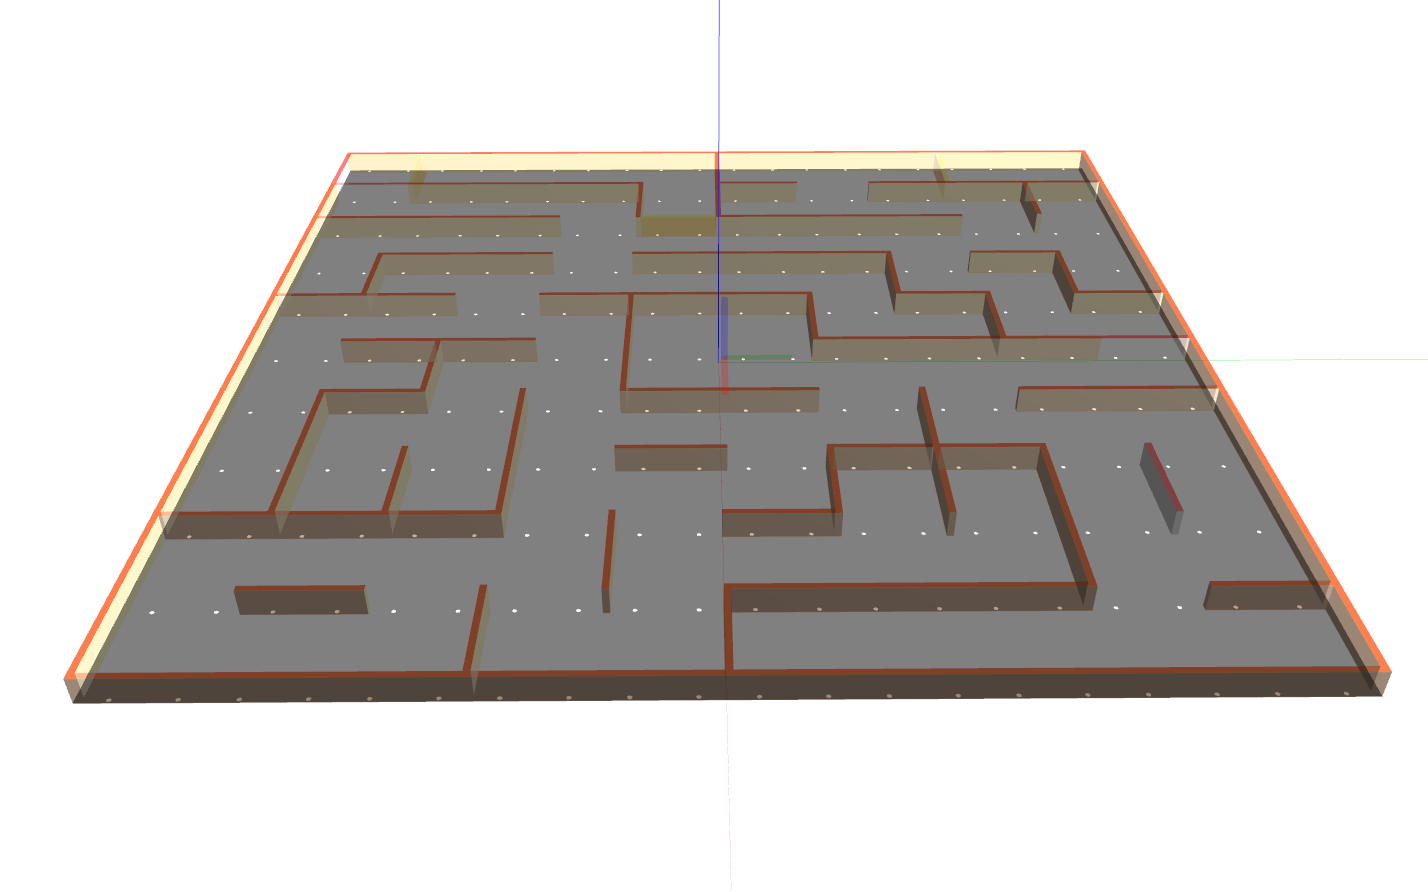
\includegraphics[scale=0.25]{minus_gazebo_colisions}}
	\label{fig:minus_gazebo_imgs}
\end{figure}

%--------- NEW SECTION ----------------------
\section{Estrutura de Software}
\label{sec:resultado_estrutura_de_software}
Para contemplar o objetivo do projeto, que é ser uma plataforma para aprendizagem de robótica móvel e inteligência artificial, optou-se pelo uso do \textit{framework} \gls*{ros} devido a sua capacidade de abstração de hardware e de reuso de software como já mencionado em \ref{sec:robotic_frameworks}. Diante disso, foi criada uma estrutura de software modular que pode ser visualizada na Figura \ref{fig:doogie_packages}. Essa estrutura é formada por \textit{stacks}, que são conjunto de pacotes agrupados em um mesmo local. Abaixo está descrito qual o objetivo de cada pacote dentro dessas \textit{stacks}.

\textbf{doogie\_base}:
\begin{itemize}
	\item \textbf{doogie\_algorithms}: Contém os algoritmos de inteligência que são utilizados pelo robô na resolução do labirinto;
	\item \textbf{doogie\_control}: Possui arquivos de configuração e de inicialização dos processos de controle do robô;
	\item \textbf{doogie\_description}: Abarca arquivos com a descrição do modelo do robô;
	\item \textbf{doogie\_msgs}: Compreende as estrutura de dados (.msg e .action) criadas exclusivamente para o Doogie Mouse;
	\item \textbf{doogie\_navigation}: Abrange os processos utilizados para a percepção, localização e navegação do robô dentro do labirinto. Fornece também \glspl*{api} para permitir que usuários implementem sua própria estratégia de resolução de labirinto.   
\end{itemize}
	
\textbf{doogie\_simulator}:
\begin{itemize}
	\item \textbf{doogie\_gazebo}: Integra todos os arquivos de configuração necessários para executar o ambiente de simulação.
\end{itemize}
	
\textbf{doogie\_robot}
\begin{itemize}
	\item \textbf{doogie\_bringup}: Agrupa arquivos de configuração e inicialização de todos os subsistemas do robô. Contém também os executáveis responsáveis pela atuação da plataforma móvel.  
	\item \textbf{doogie\_drivers}: Compreende executáveis e bibliotecas dos componentes de hardware do robô (motor, Encoder, \gls*{imu} e sensores infravermelho).
\end{itemize}
	
\textbf{doogie\_desktop}
\begin{itemize}
	\item \textbf{doogie\_rviz}: Engloba arquivos de configuração e inicialização para visualização de dados do robô no visualizador RViz;
	\item \textbf{doogie\_welcome}: Contém executáveis para verificação do funcionamento do \textit{framework} ROS na etapa de instalação.
\end{itemize}

\begin{figure}[H]
	\centering
	\caption{Organização dos pacotes do Doogie Mouse.}
	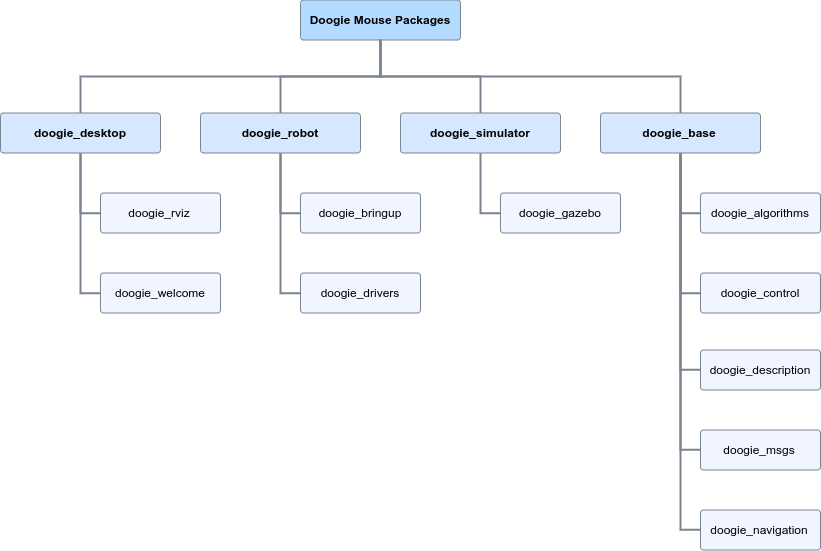
\includegraphics[width=1\textwidth]
	{Figures/doogie_packages}
	\label{fig:doogie_packages}
	\source{Própria Autoria}
\end{figure}

Dentre as \textit{stacks} e pacotes listados na Figura \ref{fig:doogie_packages} apenas a \textit{stack} doogie\_desktop e o pacote doogie\_rviz não foram criados. Os demais estão disponíveis para utilização no repositório remoto GitHub.

Embora todos esses pacotes tenham sido criados, nem todos eles são empregados no funcionamento da plataforma móvel. Como alguns pacotes são utilizados apenas para simulação do robô, não há a necessidade da sua utilização dentro da plataforma. Dessa forma, os pacotes foram organizados de acordo com o propósito final: utilização no ambiente de simulação, no robô físico ou em ambos. A Figura \ref{fig:diagrama_dos_pacotes} demonstra como esses pacotes se relacionam entre si. A \textit{stack} doogie\_base é comum tanto ao ambiente de simulação quanto ao robô físico, porém, não tem utilidade se não utilizada dentro desses dois contextos. A \textit{stack} doogie\_robot possui todos os pacotes essenciais para o funcionamento do robô físico, entretanto, possui dependência direta com a \textit{stack} doogie\_base. Em oposição está a \textit{stack} doogie\_simulator válida apenas para uso do ambiente de simulação, mas igualmente a doogie\_robot, depende da doogie\_base para funcionar. Englobando todas as \textit{stacks} mencionadas bem como a reunião de toda a documentação do robô está a \textit{stack} doogie\_desktop. A relação de dependência entre esses pacotes é feita através de arquivos de configuração que são utilizados no processo de compilação dos pacotes através de ferramentas específicas do \textit{framework} ROS. Caso uma dependência não seja satisfeita, por exemplo uma \textit{stack} não instalada, um erro ocorrerá.   

\begin{figure}[H]
	\centering
	\caption{Relação de dependência das \textit{stacks} do Doogie Mouse.}
	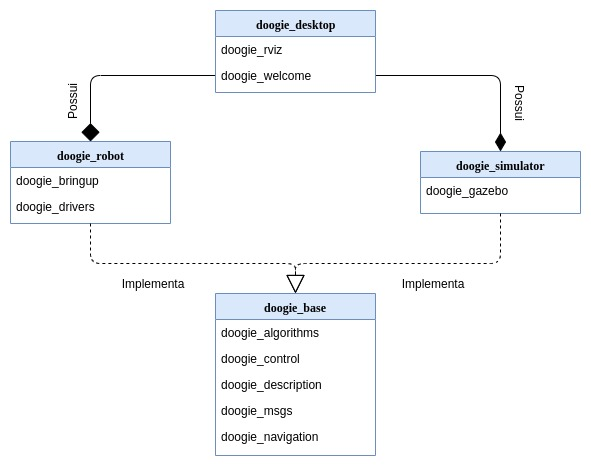
\includegraphics[width=1\textwidth]
	{Figures/diagrama_dos_pacotes}
	\label{fig:diagrama_dos_pacotes}
	\source{Própria Autoria}
\end{figure}

Continuando com a proposta de modularidade de sistemas para proporcionar um grau de flexibilidade no uso de diferentes estratégias de resolução do labirinto, foi pensado, embora não testado, um modelo de comunicação entre os processos dentro do ambiente \gls*{ros}, conforme ilustrado pela Figura \ref{fig:doogie_ros_graph}.

\begin{figure}[H]
	\centering
	\caption{Diagrama de comunicação entre processos.}
	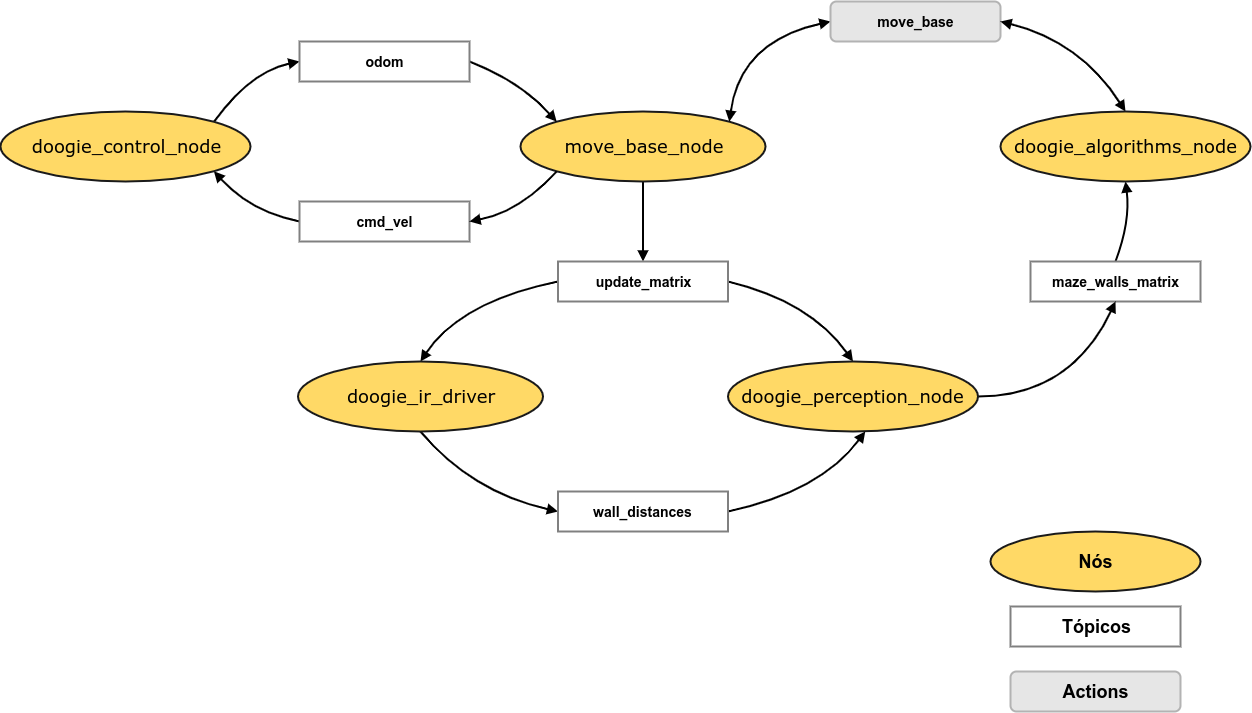
\includegraphics[width=1\textwidth]
	{Figures/doogie_ros_graph}
	\label{fig:doogie_ros_graph}
	\source{Própria Autoria}
\end{figure}

Partindo da premissa que a posição e orientação inicial da base móvel dentro do labirinto é conhecida, a movimentação do robô começa com o doogie\_algorithms\_node enviando um comando de movimentação para o move\_base\_node. Após interpretado qual movimento a plataforma deve executar, o processo move\_base\_node enviará valores de velocidade linear e angular através do tópico cmd\_vel para o processo responsável pelo controle de movimentação do robô. Com o \textit{feedback} de Odometria, o move\_base\_node infere se o robô chegou ao destino desejado. Enquanto o robô está se movimentando, uma informação de progresso é enviada para o doogie\_algorithms\_node de modo que ações possam ser tomadas enquanto o robô se locomove, como emitir uma alerta sonoro quando 90\% do trajeto for concluído																																																																																																																																																																																																																																																																																					.Quando o robô chega ao seu destino final (uma determinada célula do labirinto), uma informação de posição e orientação do robô é fornecida através do tópico update\_matrix. Essa informação é armazenada pelo processo de percepção e dispara também uma requisição para que os dados dos sensores infravermelhos sejam fornecidos. Após a requisição de dados, o \textit{driver} dos sensores infravermelho irá providenciar no tópico wall\_distances as informações de distância das paredes do labirinto. Com os valores de distância, posição e orientação do robô, o processo doogie\_perception\_node sintetiza uma matriz de obstáculos fornecendo em relação a um referencial global quais paredes existem para cada célula do labirinto visitada. Essa matriz é então fornecida para o processo que contém a estratégia de resolução do labirinto escolher a próxima ação de movimentação do robô. Essas etapas se repetem até que o robô encontre o centro do labirinto.

Com essa proposta de organização de comunicação entre processos e de posse das \glspl*{api} fornecidas para envio de comandos de movimentação do robô e manuseio da matriz de obstáculos, o usuário pode implementar sua própria estratégia de resolução de labirinto. O fator limitante de qual abordagem dentro da IA utilizar será apenas o poder de processamento da Raspberry Pi.